\documentclass[11pt]{article}
\usepackage[spanish]{babel}
\usepackage[T1]{fontenc}
\usepackage{amsmath,amsfonts,amssymb}
\usepackage{amsfonts}
\usepackage{graphicx}
\usepackage{amssymb}
\usepackage{geometry}
\usepackage{newpxtext,euler}
\usepackage{mathrsfs}
\usepackage{xcolor}
\usepackage{geometry}
 \geometry{
 a4paper,
 total={170mm,245mm},
 left=20mm,
 top=30mm,
 }
\pagestyle{empty}

\title{Taller I}

\author{Bourbaki}
\date{\today}


\begin{document}
\maketitle
\begin{enumerate}
  \item Representar gráficamente:
\end{enumerate}

$$
(1-2 i)+(-3+i) ; \quad(2+i)(-1+2 i) ; \quad \frac{-2+4 i}{1-3 i}.
$$

Note que:

\begin{align*}
  \frac{-2+4 i}{1-3 i}=\frac{-2+4 i}{1-3 i}\frac{(1+3i)}{(1+3i)}=\frac{(-2+4i)(1+3i)}{10}=-\frac{7}{5}-\frac{i}{5}
\end{align*}
y con eso se obtiene la gráfica chingona
\begin{center}
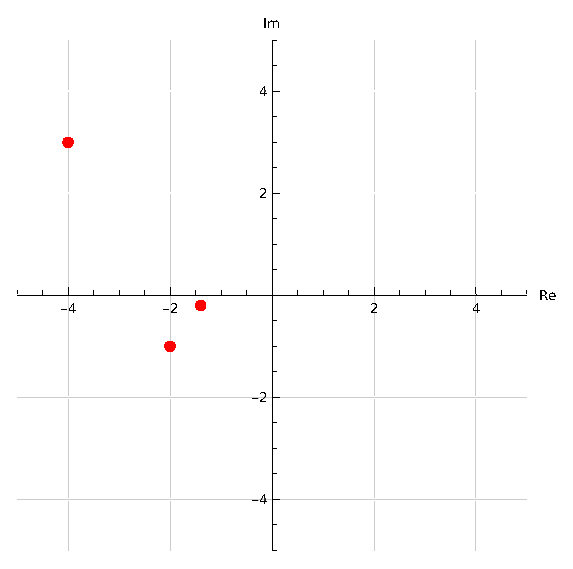
\includegraphics[scale=0.8]{Punto1}
\end{center}

\begin{enumerate}
  \setcounter{enumi}{1}
  \item Calcular el argumento principal, y escribir en forma polar $z=\dfrac{(1-i \sqrt{3})^{7}}{(\sqrt{3}-i)^{3}}$.\\

Haciendo unas cuenticas todas cacorras pero que irá a hacer su puta madre

$$z = \frac{(1 - i \sqrt{3})^7}{(\sqrt{3} - i)^3} = \frac{(1 - i \sqrt{3})^7 (\sqrt{3} + i)^3}{((\sqrt{3} - i)(\sqrt{3} + i))^3} = \frac{(1 - i \sqrt{3})^7 (\sqrt{3} + i)^3}{64} = 8i + 8\sqrt{3},
$$

luego el argumento principal es $\arctan\left(\displaystyle\frac{1}{\sqrt{3}}\right)$, además $\sqrt{8^2+8^2\times 3}=16$, esto es

$$z=16exp\left(i\frac{\pi}{6}\right),$$

pero pues yo soy un guevon y no me acordé de que es más fácil elevar cuando el número está en forma polar, entonces

$$z=\frac{(2exp(i\arctan(-\sqrt{3})))^7}{(2exp(i\arctan(-1/\sqrt{3})))^3}=2^4exp(i(7\arctan(-\sqrt{3})-3\arctan(-1/\sqrt{3}))),$$
 
 y en efecto $7\arctan(-\sqrt{3})-3\arctan(-1/\sqrt{3})+2\pi=\dfrac{\pi}{6}$

  \item Mostrar que el triangulo de vertices $z_{1}, z_{2}, z_{3}$ es equilatero, si y solo si
\end{enumerate}

$$
z_{1}^{2}+z_{2}^{2}+z_{3}^{2}=z_{1} z_{2}+z_{2} z_{3}+z_{3} z_{1}
$$

Para este punto primero note que dado un triángulo equilatero, podemos escribir a sus vértices de la forma

$$z_1=r^{1/3}exp\left(\dfrac{i\theta_1}{3}\right)+w, \quad z_2=r^{1/3}exp\left(\dfrac{i\theta_2}{3}\right)+w \quad \text{y}\quad z_3=r^{1/3}exp\left(\dfrac{i\theta_3}{3}\right)+w,$$

con $w\in \mathbb{C}$, luego los vértices del triángulo equilátero son soluciones del polinomio $(z-a)^3-b=0=(z-z_1)(z-z_2)(z-z_3)$, en efecto

\begin{align*}
  (z-z_1)(z-z_2)(z-z_3)&=z^3-z^2(z_2+z_1+z_3)+z(z_1z_2+z_2z_3+z_1z_3)-z_1z_2z_3\\
  &=(z-a)^3-b\\
  &=z^3-z^2(3a)+z(3a^2)-b-a^3
.\end{align*}

Ahora comparando coeficientes obtenemos que $3a=z_1+z_2+z_3$ y $3a^2=z_1z_2+z_2z_3+z_1z_3$, esto es 

$$3(z_1z_2+z_2z_3+z_1z_3)=(z_1+z_2+z_3)^2$$

de donde se sigue la equivalencia deseada.

\begin{enumerate}
  \setcounter{enumi}{3}
  \item Mostrar que la suma de los angulos interiores de un triangulo es $\pi$

  Sean $z_1,z_2,z_3\in \mathbb{C}$ vertices de un triangulo cualquiera y $\theta_1,\theta_2,\theta_3\in[0,\pi)$ los respectivos angulos. Primero note que si trasladamos el triangulo tal que el vertice $z_1$ quede sobre el origen, los vertices del triangulo en sentido antihorario son $0,z_2-z_1$ y $z_3-z_1.$ donde el angulo entre estos dos vectores sigue siendo $\theta_1$ ya que trasladar no afecta los angulos. Recordemos que $e^{i\theta_1}$ rota a un vector a traves del origen el angulo $\theta_1$ en sentido antihorario, asi $(z_2-z_1)e^{i\theta_1}=r_1(z_3-z_1),$ donde $r_1$ es un factor de escalacion. Haciendo el mismo proceso para los verices $z_2$ y $z_3$ tenemos las siguientes ecuaciones
  $$\begin{cases}
    (z_2-z_1)e^{i\theta_1}=r_1(z_3-z_1),\\
    (z_3-z_2)e^{i\theta_2}=r_2(z_1-z_2),\\
    (z_1-z_3)e^{i\theta_3}=r_3(z_2-z_3).
  \end{cases}$$
  Luego 
  $$\begin{cases}
    e^{i\theta_1}=r_1\dfrac{z_3-z_1}{z_2-z_1},\\
    e^{i\theta_2}=r_2\dfrac{z_1-z_2}{z_3-z_2},\\
    e^{i\theta_3}=r_3\dfrac{z_2-z_3}{z_1-z_3}.
  \end{cases}$$
  Tomando el argumento principal en ambos lados de la ecuacion obtenemos
  $$\begin{cases}
    \theta_1=Arg\left(r_1\dfrac{z_3-z_1}{z_2-z_1}\right),\\
    \theta_2=Arg\left(r_2\dfrac{z_1-z_2}{z_3-z_2}\right),\\
    \theta_3=Arg\left(r_3\dfrac{z_2-z_3}{z_1-z_3}\right).
  \end{cases}$$
  Recordemos que el argumento del producto de dos complejos es igual a la suma de los argumentos, luego
  \begin{align*}
    \theta_1+\theta_2+\theta_3&=Arg\left(r_1\dfrac{z_3-z_1}{z_2-z_1}\right)+Arg\left(r_2\dfrac{z_1-z_2}{z_3-z_2}\right)+Arg\left(r_3\dfrac{z_2-z_3}{z_1-z_3}\right)\\
    &=Arg\left(\left(r_1\dfrac{z_3-z_1}{z_2-z_1}\right)\left(r_2\dfrac{z_1-z_2}{z_3-z_2}\right)\left(r_3\dfrac{z_2-z_3}{z_1-z_3}\right)\right)\\
    &=Arg(-r_1r_2r_3)\\
    &=Arg(r_1r_2r_3e^{i\pi})\\
    &=\pi
  \end{align*}

  \item Mostrar que
\end{enumerate}

\begin{itemize}
  \item $\sin 3 x=3 \cos ^{2} x \sin x-\sin ^{3} x$\\

En efecto

$$
\begin{aligned}
\sin (x+2 x)= & \sin x \cos 2 x+\cos x \sin 2 x \\
= & \sin x\left(\cos ^2 x-\sin ^2 x\right)+\cos x(\sin x \cos x+\cos x \sin x) \\
= & \sin x\left(1-2 \sin ^2 x\right)+2 \cos ^2 x \sin x \\
= & \sin x-2 \sin ^3 x+2 \cos ^2 x \sin x \\
= & \sin x\left(1+2 \cos ^2 x\right)-2 \sin ^3 x \\
= & \sin x\left(\sin ^2 x+3 \cos ^2 x\right)-2 \sin ^3 x \\
= & 3 \sin x \cos ^2 x-\sin ^3 x
\end{aligned}
$$

  \item $\cos 3 x=\cos ^{3} x-3 \cos x \sin ^{2} x$\\

  En efecto

  $$
\begin{aligned}
\cos (x+2 x) & =\cos x \cos 2 x-\sin x \sin 2 x \\
& =\cos x\left(\cos ^2 x-\sin ^2 x\right)-2 \sin x(\sin x \cos x) \\
& =\cos ^3 x-\cos x \sin ^2 x-2 \sin ^2 x \cos x \\
& =\cos ^3 x-3 \sin ^2 x \cos x
\end{aligned}
$$
  \item $\cos 8 x+28 \cos 4 x+35=64\left(\cos ^{8} x+\sin ^{8} x\right)$\\

  Recordemos que $\sin^2x+\cos^2x=1,$ luego $\sin^4x+\cos^4x+2\sin^2x\cos^2x=1$ \textcolor{blue}{Luego sigo me dio pereza hacer esto :p}

\end{itemize}

\begin{enumerate}
  \setcounter{enumi}{5}
  \item Graficar las raices cuartas de $i,-16,-2+2 i \sqrt{3}$

En este solo vamos a poner el último porque el Sercoya dijo que todos son cuadrados (ese es el rey de la pedancia), además los otros ejercicios son iguales, note que

$$r=\sqrt{4+4\times 3}=4 \quad \text{ además } \theta=\arctan\left(-\sqrt{3}\right) +\pi=\frac{2\pi}{3},$$

de esto se sigue que los puntos son de la forma

$$z=exp\left(i\frac{\left(\dfrac{2\pi}{3}+2\pi k\right)}{4}\right) , \quad k=0,1,2,3.$$
Obtenemos la gráfica chingona 

\begin{center}
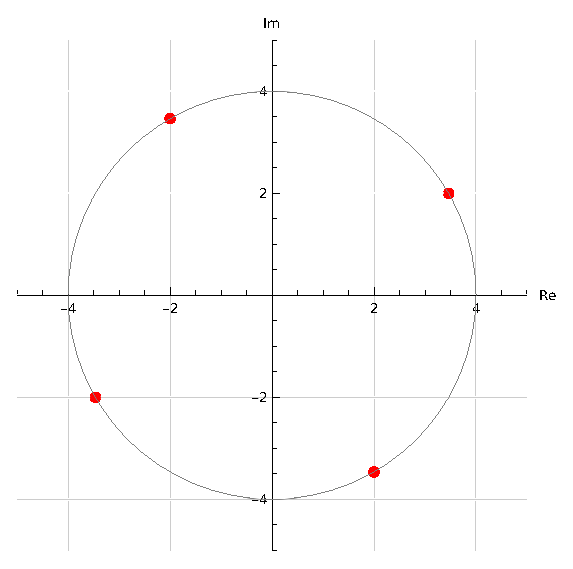
\includegraphics[scale=0.8]{Punto6.eps}
\end{center}

  \item Resolver la ecuación $z^{10}+4=0$

Note que $z^{10}=4e^{i\pi}$, entonces las soluciones son de la forma 

$$z=4^{\frac{1}{10}}exp\left(i\left(\displaystyle\frac{\pi+2\pi k}{10}\right)\right) \quad k=0,\ldots,9$$

y pues para rellenar espacio mire otra chingona

\begin{center}
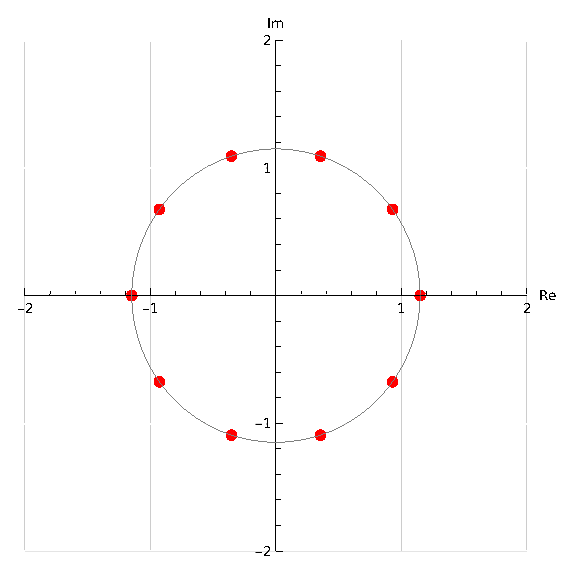
\includegraphics[scale=1]{Punto7.eps}
\end{center}

  \item Mostrar que las raices de la ecuación $(z+1)^{5}+z^{5}=0$, estan sobre la recta $x=-\frac{1}{2}$

Note que la ecuación se puede escribir como

$$\left(\frac{z+1}{z}\right)^5=-1=exp(i\pi)$$

de donde se sigue que $\dfrac{z+1}{z}=w=exp\left(i\left(\dfrac{\pi+2\pi k}{5}\right)\right)$ con $k=0,\ldots,4$, en efecto

$$\Re(z)=\Re\left(\frac{1}{w-1}\right)=\Re\left(\frac{\overline{w}-1}{|w-1|^2}\right)$$

tomando $w=a+bi$ y sabiendo que $|w|=1$ se sigue que

$$\Re(z)=\Re\left(\frac{a-bi-1}{(a-1)^2+b^2}\right)=\frac{a-1}{(a-1)^2+b^2}=\frac{a-1}{a^2-2a+1+b^2}=\frac{a-1}{2(1-a)}=-\frac{1}{2}$$

  \item Mostrar que para $n \neq 0$, las raices de la ecuación $(1+z)^{2 n}+(1-z)^{2 n}=0$, estan dadas por
\end{enumerate}

$$7\arctan(-\sqrt{3})-3\arctan(-1/\sqrt{3})
z_{k}=i \tan \frac{(2 k+1) \pi}{4 n} n \in \mathbb{Z}^{+}, \quad k=0,1,2, \ldots
$$

\begin{enumerate}
  \setcounter{enumi}{9}
  \item Calcular $(-3+4 i)^{\frac{3}{2}}$, primero tomando la raíz cuadrada y el resultado elevarlo al cubo, y segundo, invirtiendo el procedimiento.\\

  Note que

$$z^{1/2} = \sqrt{5} \, \exp \left( \frac{i}{2} \left( \pi + \arctan \left( -\frac{4}{3} \right) + 2 \pi k \right) \right), \quad k = 0, 1$$

$$z_0^{3/2}= 5 \sqrt{5} \, \exp \left( \frac{3i}{2} \left( \pi + \arctan \left( -\frac{4}{3} \right) \right) \right), \quad z_1^{3/2} = 5 \sqrt{5} \, \exp \left( \frac{3i}{2} \left( \pi + \arctan \left( -\frac{4}{3} \right) + 2 \pi \right) \right)$$

Por otro lado

$$z^3 = 5^3 \, \exp \left( 3i \left( \pi + \arctan \left( -\frac{4}{3} \right) \right) \right)$$

$$z_0^{3/2}= 5 \sqrt{5} \, \exp \left( \frac{3i}{2} \left( 3 \pi + \arctan \left( -\frac{4}{3} \right) \right) \right),\quad z_1^{3/2} = 5 \sqrt{5} \, \exp \left( \frac{3i}{2} \left( \pi + \arctan \left( -\frac{4}{3} \right) + 2 \frac{\pi}{3} \right) \right)
$$

Se puede ver que en efecto en este caso da igual el orden de tomar la potencia dado que al distribuir $\dfrac{3}{2}$ en las expresiones anteriores obtenemos por un lado un ángulo $\phi+3\pi$ y por el otro $\phi+\pi$ que sabemos que son el mismo ángulo, esto pasa  porque 3 y 2 son primos relativos xd.\\

Toca acordarse de que $\left(z^{1/n}\right)^m$ tiene menos elementos que $\left(z^{m}\right)^{1/n}$ si $(m,n)> 1$

  \item Calcular $(-3+4 i)^{-\frac{3}{2}}$.

  Sea $z=(-3+4i)$, note que $z^{-3}=\dfrac{1}{125} exp\left( i \left(-3\pi +3\arctan\left(\dfrac{4}{3}\right)\right)\right)$, entonces


$$z^{-3/2}=\dfrac{\sqrt{5} }{25} exp\left( \frac{i}{2} \left(-3\pi +3\arctan\left(\dfrac{4}{3}\right)+2\pi k\right)\right), \quad k=0,1$$
\end{enumerate}

\end{document}